\documentclass[11pt, a4paper]{article}
\usepackage[utf8]{inputenc}
\usepackage{geometry}
\geometry{a4paper, margin=1in}
\usepackage{graphicx}
\usepackage{amsmath}
\usepackage{amsfonts}
\usepackage{booktabs}
\usepackage{hyperref}
\hypersetup{hypertexnames=false}
\usepackage{float}

\title{\textbf{Principles of Artificial Intelligence --- Homework 4}}
\author{
    \textbf{Student ID:} 112511059, 112511089
}
\date{\today}

\begin{document}

\maketitle

\section{Maximizing the Reward}

The empirical evaluation of the three core multi-armed bandit (MAB) algorithms yielded distinct exploitation-exploration behaviors across 1,000 trials:

\begin{figure}[H]
    \centering
    
\includegraphics[width=0.8\textwidth]{../results/part1.png}
    % \path{../results/part1.png} % Placeholder for image path
    \caption{Performance Overview of the Three MAB Algorithms}
    \label{fig:part1}
\end{figure}

\begin{itemize}
    \item \textbf{$\epsilon$-Greedy ($\epsilon = 0.5$):} Due to a high and rigidly fixed exploration rate of 50\%, a substantial number of trials were wasted on suboptimal arms (Arm 0 and Arm 1 were pulled over 160 times each). Consequently, this algorithm generated the highest cumulative regret among the three baseline methods.
    \item \textbf{Upper Confidence Bound (UCB with $C = 0.5$):} In this baseline, an algorithmic misuse occurred where the cumulative empirical reward ($\text{Wins} \times 20$) was used instead of the true empirical win rate. This caused the reward term to heavily outweigh the confidence bound. Following a single early win, Arm 2 completely dominated the index calculation, plunging the model into decisive exploitation prematurely. Although this specific random seed happened to yield the highest total wins (808 wins), it poses a severe risk of premature convergence in general scenarios.
    \item \textbf{Thompson Sampling:} This algorithm demonstrated the most elegant dynamic balance between exploration and exploitation. After sampling merely 3 trials, it decisively abandoned the poorly performing Arm 0. Following a well-justified exploration of Arm 1, it robustly locked onto the true optimal arm (Arm 2, with 821 pulls). Its posterior Beta distribution also emerged as the most concentrated, reflecting high statistical certainty.
\end{itemize}

\section{Hyperparameter Selection}

\subsection{\texorpdfstring{$\epsilon$}{epsilon}-Greedy Variants}

\subsubsection{Uniform \texorpdfstring{$\epsilon$}{epsilon}}
Maintaining a fixed exploration probability highlights a fundamental trade-off: setting $\epsilon$ too small ($\epsilon < 0.02$) prevents sufficient exploration, leaving the agent trapped in local optima. Conversely, setting $\epsilon$ too high ($\epsilon > 0.5$) degrades the model into a random gambler that chooses blindly, both extremes leading to a significant drop in total wins.

\begin{figure}[H]
    \centering
    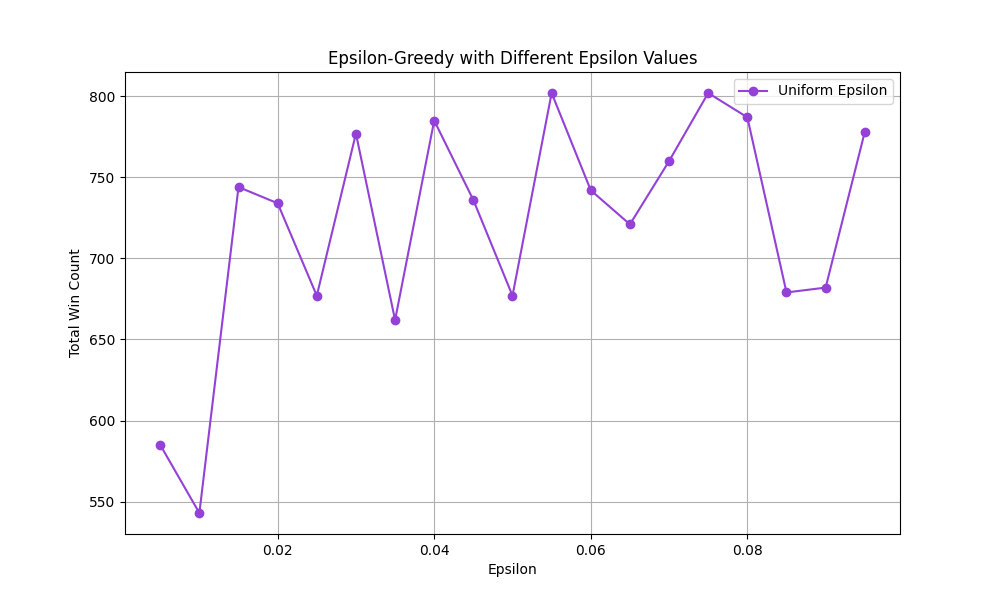
\includegraphics[width=0.45\textwidth]{../results/uniform_epsilon_greedy.png}
    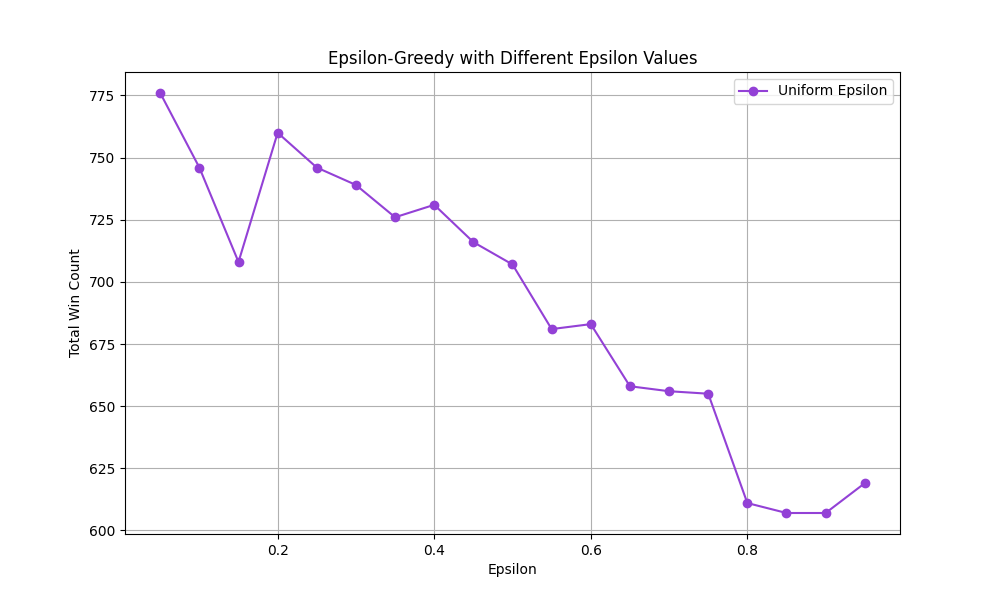
\includegraphics[width=0.45\textwidth]{../results/uniform_epsilon_greedy_1.png}
    % \path{../results/uniform_epsilon_greedy.png} \quad \path{../results/uniform_epsilon_greedy_1.png}
    \caption{Impact of Uniform Exploration Rates on Performance}
\end{figure}

\subsubsection{Time-Descending \texorpdfstring{$\epsilon$}{epsilon}}
Implementing a time-dependent decay for $\epsilon$ consistently improves the performance of the multi-armed bandit across various settings. This validates the foundational principle that an "aggressive exploration in the early phase, followed by focused exploitation in the late phase" strategy resolves the exploration-exploitation dilemma more effectively.

\begin{figure}[H]
    \centering
    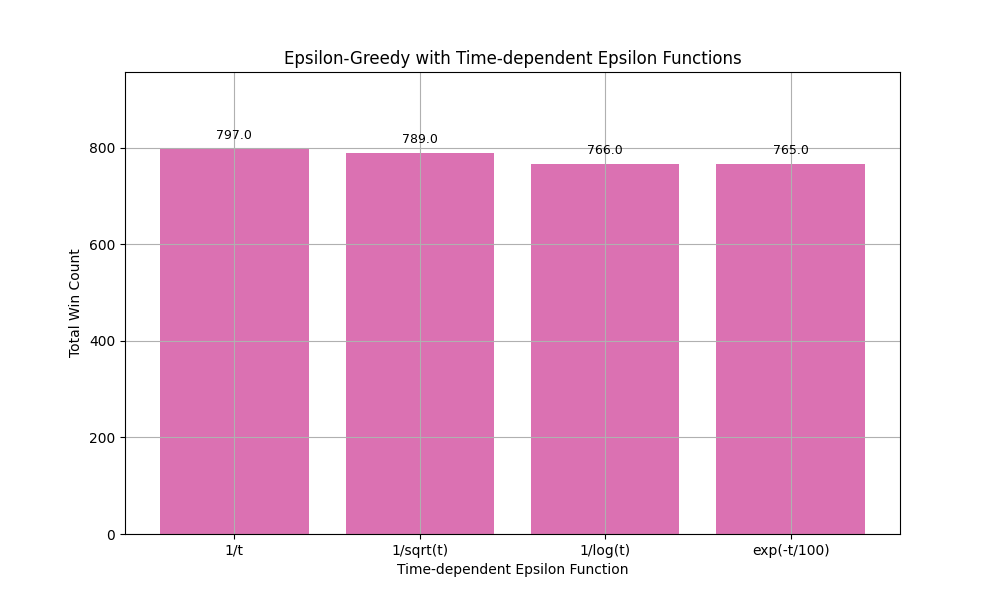
\includegraphics[width=0.7\textwidth]{../results/time_dependent_epsilon_greedy.png}
    % \path{../results/time_dependent_epsilon_greedy.png}
    \caption{Performance Trend of Time-Descending Exploration}
\end{figure}

\subsubsection{Insights on the Scaling of Exponential Decay}
Because exponential functions decay much faster than polynomial functions, the scaling constant $s$ within the exponent heavily dictates the final performance. In extreme configurations, setting $s$ to the total number of trials (\texttt{NUM\_TRIAL}) over-prolongs the exploration phase, whereas setting $s=1$ makes the model's trajectory overly sensitive to the initial arm selections. Therefore, this parameter demands careful tuning.

\begin{figure}[H]
    \centering
    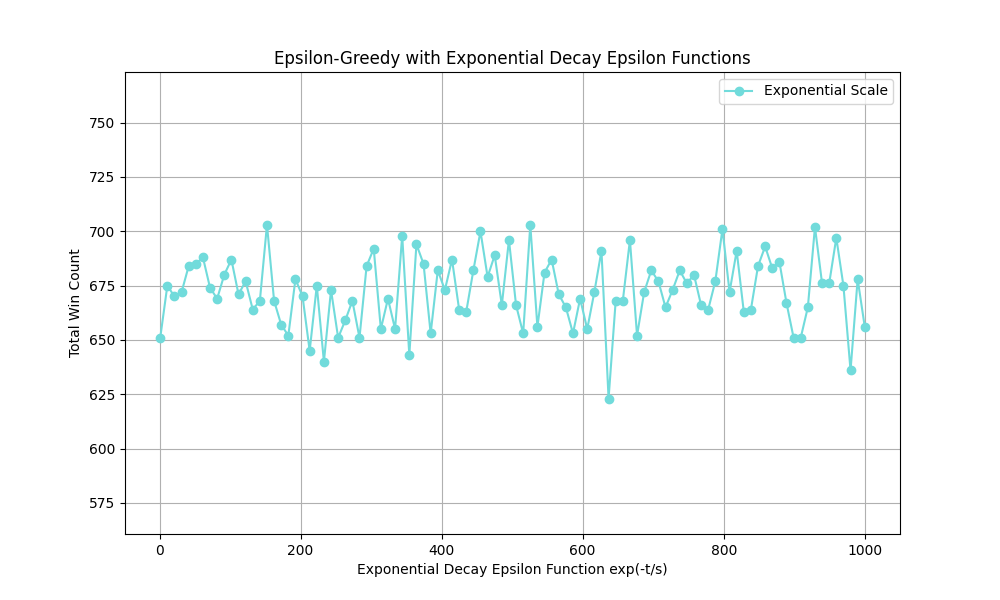
\includegraphics[width=0.7\textwidth]{../results/exponential_decay_epsilon_greedy.png}
    % \path{../results/exponential_decay_epsilon_greedy.png}
    \caption{Sensitivity Analysis of Exponential Decay Scaling Parameters}
\end{figure}

\subsection{Upper Confidence Bound (UCB)}

\subsubsection{Adjusting the UCB Formula}
To correct the scaling mismatch observed in Section 1, the formula's value term was modified from "average absolute reward" to "empirical win rate". This adjustment prevents the reward magnitude from dominating the confidence term, which previously suppressed exploration. This calibrated formulation successfully encourages the model to explore more actively during the initial steps, although under this specific framework, it did not outperform the edge-case success of the uncalibrated baseline.

\begin{figure}[H]
    \centering
    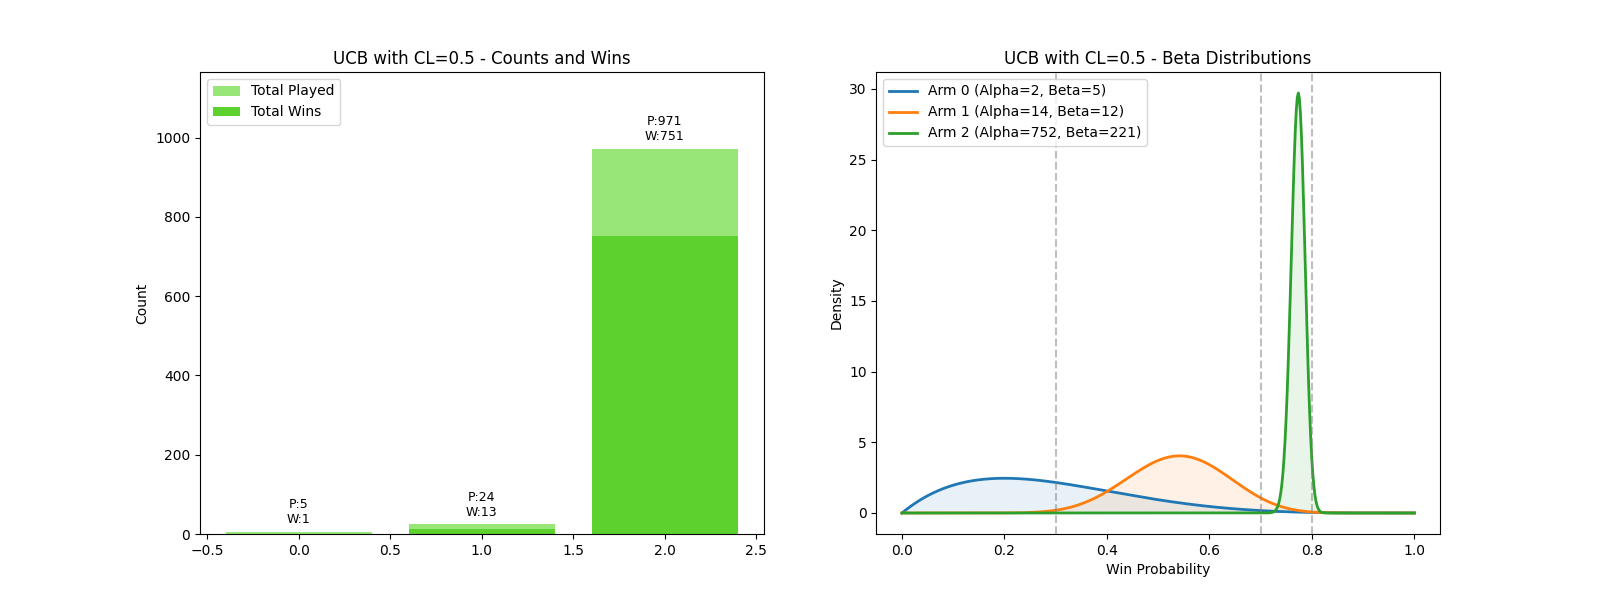
\includegraphics[width=0.7\textwidth]{../results/ucb_cl_0.5.png}
    % \path{../results/ucb_cl_0.5.png}
    \caption{Performance of the Calibrated UCB Algorithm ($C=0.5$)}
\end{figure}

\subsubsection{Testing the Sensitivity of the Confidence Level \texorpdfstring{$C$}{C}}
The exploration constant $C$ plays a pivotal role in performance. Optimal results are achieved when $C$ ranges between $0.3 \sim 0.8$, a window that effectively prevents premature convergence while allowing rapid transition into exploitation, yielding high win counts of roughly $780 \sim 800$. As $C$ scales higher, the model suffers from over-exploration, which progressively penalizes and lowers the total win count.

\begin{figure}[H]
    \centering
    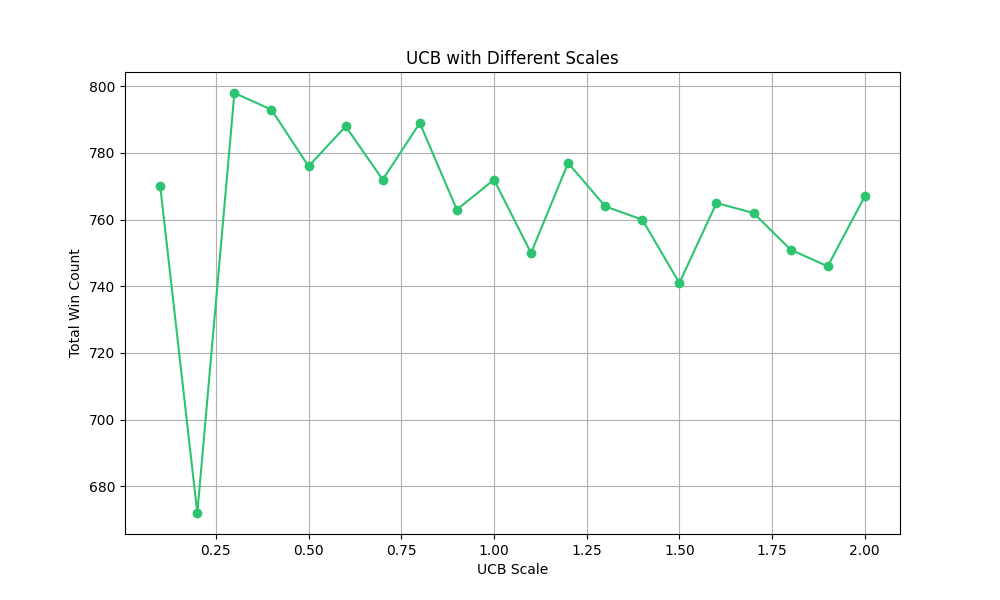
\includegraphics[width=0.7\textwidth]{../results/ucb_scales.png}
    % \path{../results/ucb_scales.png}
    \caption{Sensitivity Analysis of the Exploration Constant $C$ in UCB}
\end{figure}

\subsection{Thompson Sampling with Varied Priors}
By systematically varying the $(\alpha, \beta)$ hyperparameter pairs across 100 different combinations, the resulting win-count heatmap reveals that the vast majority of combinations yield scores that align closely with the theoretical optimum.

\begin{figure}[H]
    \centering
    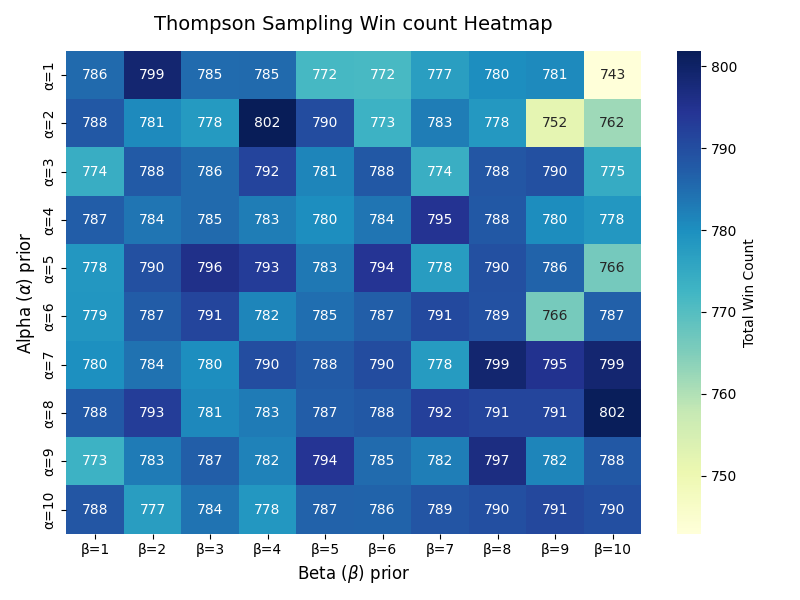
\includegraphics[width=0.7\textwidth]{../results/Thompson_sampling_varing_prior.png}
    % \path{../results/Thompson_sampling_varing_prior.png}
    \caption{Heatmap of Total Win Counts for Thompson Sampling under Varied Priors}
\end{figure}

To determine the mathematical significance of these variations, a one-way ANOVA was conducted across the 100 distinct groups. The statistical test confirmed that under extremely pessimistic priors (located in the upper-right corner where $\alpha \ll \beta$), the model spends an excessive number of early steps correcting its initial bias. Consequently, its final cumulative performance within the 1,000-step horizon is significantly compromised. 
$$\text{F-statistic} = 1.6735, \quad p\text{-value} = 9.9439 \times 10^{-5}$$
Given that the $p\text{-value} < 0.05$, we reject the null hypothesis, concluding that prior distributions do have a statistically significant effect on the final performance under extreme constraints.

\section{Conclusion}

Based on our empirical analysis, we draw the following conclusions regarding the three multi-armed bandit approaches:
\begin{enumerate}
    \item[(a)] \textbf{$\epsilon$-Greedy} is fundamentally inefficient due to its rigid, history-agnostic exploration strategy which wastes trials even after the optimal arm is clear.
    \item[(b)] \textbf{UCB} achieves strong performance but is highly fragile, relying heavily on "scale alignment" between the objective reward magnitudes and the exploration constant $C$.
    \item[(c)] \textbf{Thompson Sampling} leverages Bayesian posterior updates to establish the most robust, self-correcting dynamic balance. It reaches optimal convergence efficiently without requiring tedious hyperparameter tuning.
\end{enumerate}

\end{document}